\section{Some analysis in one dimension}\label{sec:theory}


We study some accuracy and stability properties of the finite volume method stabilized with the state redistribution method on uniform and nonuniform grids in one dimension, on which we solve
$$
u_t + a u_x = 0,
$$
with periodic boundary conditions.  
The uniform grid is composed of $N$ cells with size $h = \frac{1}{N}$.  Merging neighborhoods are composed of an odd number cells, centered on cell $i$, e.g., the tile made of three cells, associated with cell $i$ is contains cells $i-1$, $i$, and $i+1$ (figure \ref{fig:overlapping1D}).
More generally, the merging neighborhood of width $k$ has is composed of $2k+1$ cells.
\begin{figure}
    \centering
    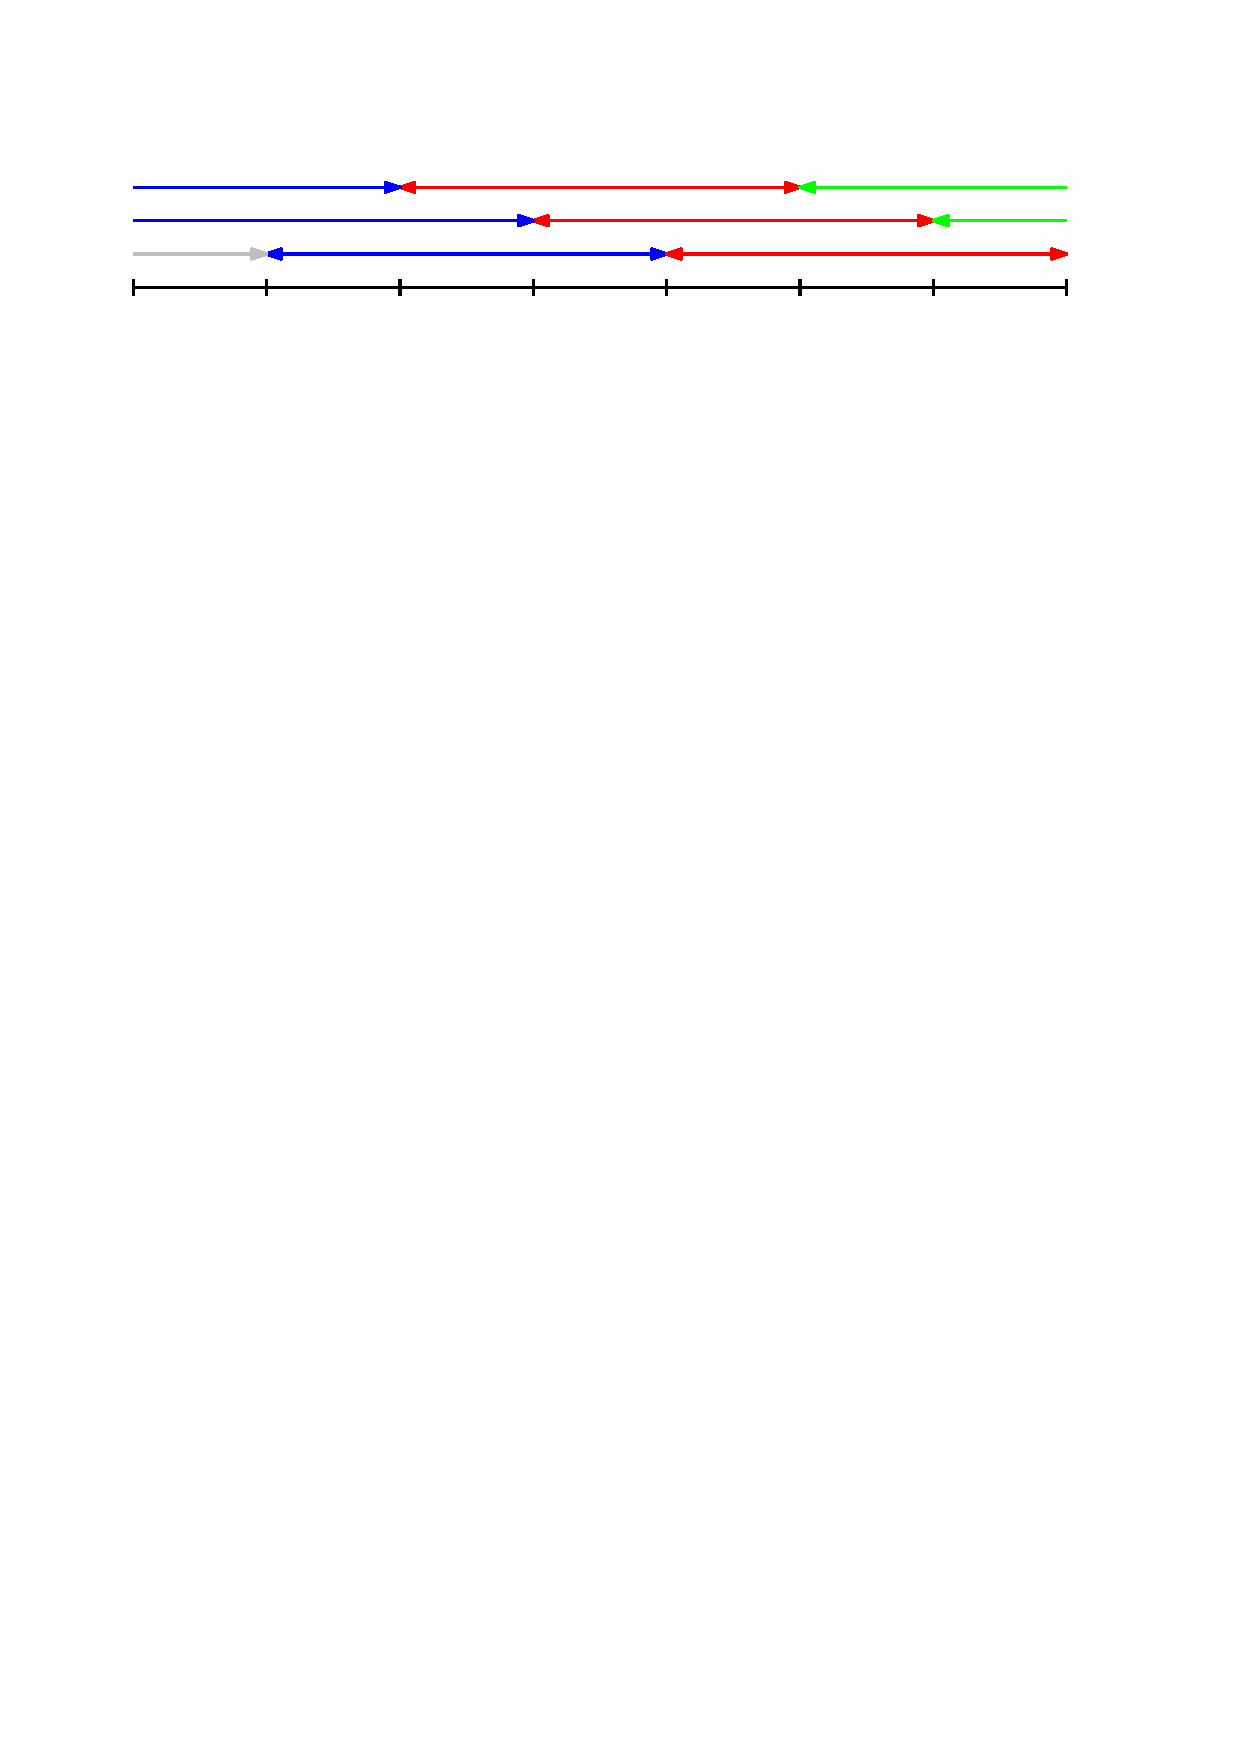
\includegraphics[width = 0.8\textwidth]{figs/overlapping1D.pdf}
    \caption{Overlapping neighborhoods on the uniform grid composed of three cells of width $k=1$.}
    \label{fig:overlapping1D}
\end{figure}
The nonuniform grids are composed of $N$ randomly generated cells.

\subsection{Truncation error}
The truncation error is
$$
\tau = \frac{u^{n+1}- L(u^n)}{\Delta t},
$$
where $u^n$ is a grid function of the exact solution at time $t^n$, and $L$ is finite volume update stabilized by the state redistribution method.  
When the scheme is stable, the truncation error can describe the order of accuracy of the finite volume method.
On uniform grids, a simple calculation shows that the truncation error is $||\tau|| = \mathcal{O}(h^{p+1})$.  On nonuniform grids, the truncation error is $||\tau|| = \mathcal{O}(h^{p})$.  This is a well-known phenomenon for schemes on nonuniform grids.
In figure \ref{fig:truncationerror}, we provide a convergence plot of the truncation error for various orders of approximation on uniform and nonuniform grids.
\begin{figure}
    \centering
\subfloat[]{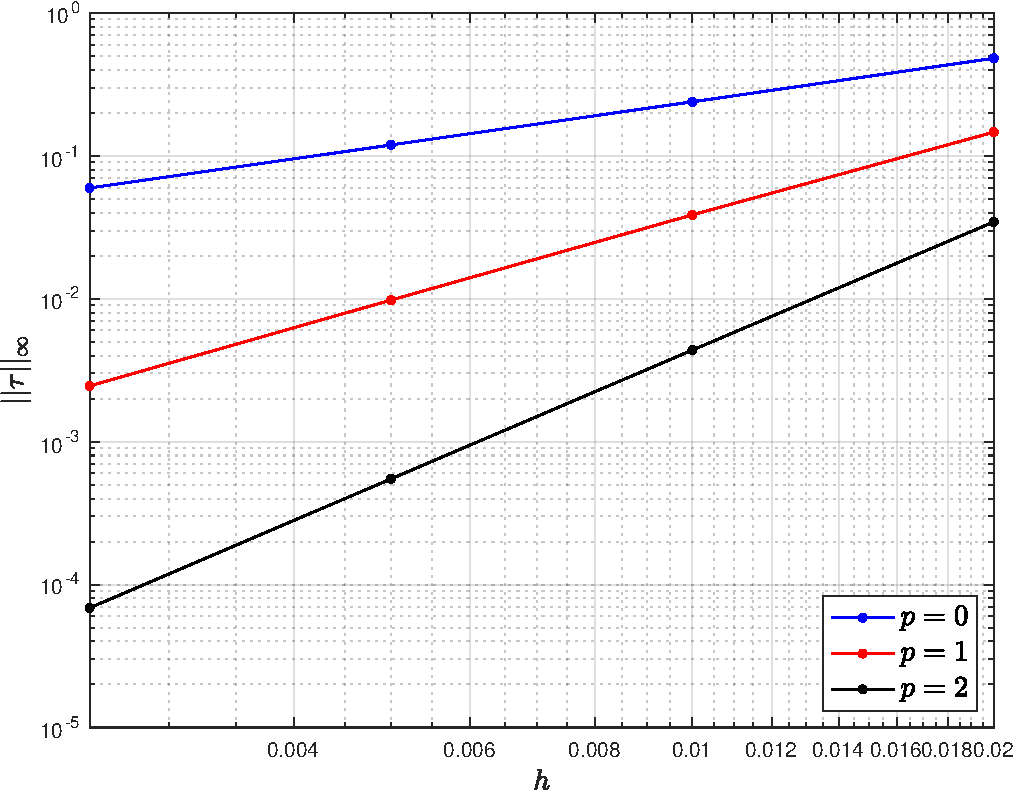
\includegraphics[width=0.45\linewidth]{figs/truncationerror_uniform.pdf}} \hfill
\subfloat[]{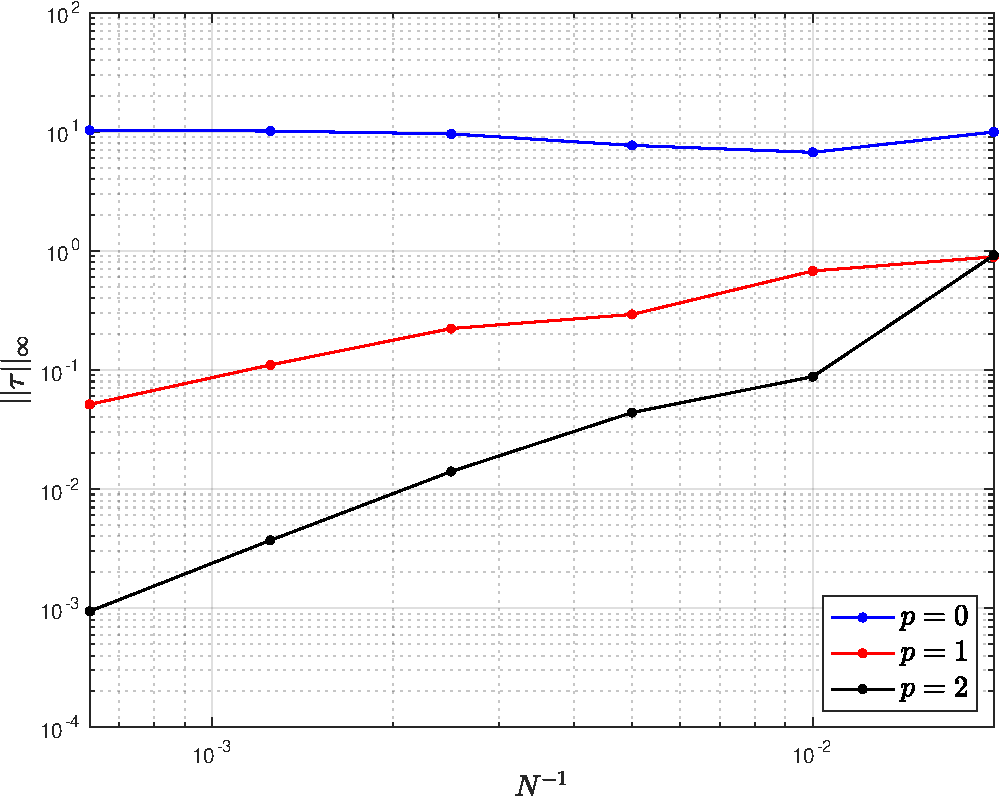
\includegraphics[width=0.45\linewidth]{figs/truncationerror_nonuniform.pdf}}
    \caption{Influence of the merging neighborhood size and the merging tile size on the CFL number.  SHOULD I DID POINTWISE VALUES EVEN FOR P=2 HERE..SHOULD FIX THAT.}
    \label{fig:truncationerror}
\end{figure}
On nonuniform grids, we observe that the truncation error loses an order of accuracy.  However, numerical examples in section \ref{sec:compResults} demonstrate that the scheme does not.

\subsection{Eigenvalue stability}
The goal of this section is twofold.  First, we confirm the intuition that the maximum allowable time step restriction increases with the size of merging neighborhoods.  Next, we show that the error in the numerical solution increases with both the size of the merging neighborhood and the size of the reconstruction stencil on the neighborhood.

The finite volume update after one forward Euler time step can be written in matrix form
\begin{equation}\label{eq:L}
    \hat U = (I + \Delta t L)U^n,
\end{equation}
where $L$ is the finite volume approximation of $-a\frac{\partial u}{\partial x}$, and $\hat U = [\hat U_1, \hat U_2, \hdots, \hat U_N]$.
The next step of the SRD method can be written in matrix form
\begin{equation}\label{eq:merged_tile}
\hat Q = T\hat U,
\end{equation}
where $\hat Q = [\hat Q_1, \hat Q_2, \hdots, \hat Q_N]$, and the matrix $T$ depends on the merging neighborhood.  The matrix $T$ is circulant due to the periodic boundary conditions.  
The first row of the $T$ matrix associated with central merging tile of size $2n+1$ is
$$
\frac{1}{2n+1}[\underbrace{1, 1, \hdots,1}_{n+1}, 0, \hdots, 0,\underbrace{1, 1, \hdots, 1}_{n}].
$$
The final step of the SRD method maps the averages on the merging tiles back to the original mesh with the matrix $S$, i.e.,
% \begin{align}
%   U^{n+1}_i =  \frac{1}{J} \sum^n_{k = - n}\hat Q_{i+k} &- (\hat Q_{i+ k + n + 1}-\hat Q_{i- k - n-1})\frac{k}{J+1}\\
%   &+ (\hat Q_{i+k+n + 1} -2 \hat Q_{i+k} +\hat Q_{i-k - n-1})\left(2\frac{k^2}{(J+1)^2} - \frac{n}{3(J+1)}\right).
% \end{align}
the final update for the finite volume method without slope reconstruction is
$$
U^{n+1} = ST(I + \Delta t L)U^n.
$$
The matrix $S$ depends on whether a slope is reconstructed on the merging neighborhood or not.  
If a high-order reconstruction in the finite volume method is used, we time step using an SSP-RK method of the same order.  Since SSP-RK methods are convex combinations of forward Euler time steps, we apply the SRD method after a forward Euler step.  That is, for linear and quadratic reconstructions, the final update is
\begin{equation}
\begin{aligned}
    U^{(1)} &= ST(I + \Delta t L)U^n, \\
    U^{(2)} &= ST(I + \Delta t L)U^{(1)},\\
    U^{n+1} &= \frac{1}{2}U^n + \frac{1}{2}U^{(2)},
\end{aligned}
\end{equation}
and 
\begin{equation}
\begin{aligned}
    U^{(1)} &= ST(I + \Delta t L)U^n, \\
    U^{(2)} &=  \frac{3}{4}U^n + \frac{1}{4}ST(I+\Delta t L)U^{(1)} ,\\
    U^{(3)} &= ST(I+\Delta t L)U^{(2)}, \\
    U^{n+1} &= \frac{1}{3}U^n + \frac{2}{3}U^{(3)},
\end{aligned}
\end{equation}
respectively.  
The linear mapping from $U^n$ to $U^{n+1}$ is given by
$$
U^{n+1} = AU^n.
$$
The dominant eigenvalue of the complete scheme, $A$, is a function of $\Delta t$, and is given by
$$
\lambda(\Delta t) = \max_{i=1}^{N}|\lambda_i(\Delta t)|,
$$
where $\lambda_i$ is the $i$th eigenvalue of $A(\Delta t)$.
 We aim to compute the maximum $\Delta t$ for which $\lambda(\Delta t) \leq 1$, i.e., we want to find $\Delta t_{\text{max}}$ such that given a $\Delta t$ for which $0\leq \Delta t \leq \Delta t_{\text{max}}$, we have $\lambda(\Delta t) \leq 1$. 
 







 
%  \subsubsection*{First order method}
% The finite volume update is
% $$
% \hat U_i = U^n_i -a\frac{\Delta t}{h}(U^n_i - U^n_{i-1}),
% $$
% or, in matrix form
% $$
% \hat U = \left(I -\Delta t L \right)U^n,
% $$
% where the matrix $L$ is circulant, and its first row is
% $$
% \frac{a}{h}[1, 0, \hdots, 0, -1].
% $$
% The final solution update is
% $$
% U^{n+1}_i = \frac{1}{N_i}\sum_{k \in W_i} \hat Q_k,
% $$
% where $W_k$ is the set of merging tiles to which cell $i$ belongs.  In matrix form, this becomes
% \begin{equation}
%     U^{n+1} = S_0 \hat Q,
% \end{equation}
% where the matrix $S_0$ is circulant.  
% The first row of the $S_0$ matrix associated with the central merging tiles is
% $$
% [\underbrace{\frac{1}{2n+1}, \frac{1}{2n+1}, \hdots, \frac{1}{2n+1}}_{n+1}, 0, \hdots, 0,\underbrace{\frac{1}{2n+1}, \hdots, \frac{1}{2n+1}}_{n}],
% $$
% where $2n+1$ is the number of cells in the central merging neighborhood, since cell $i$ belongs to merging tiles to the left and right.
% The entire state redistribution algorithm is
% $$
% U^{n+1} = S_0T \left(I + a\frac{\Delta t}{h} L \right)U^n.
% $$


% % We aim to determine how large of a time step we can take in terms of the size of the merging neighborhood.
% % In Figure \ref{fig:cfl_vs_nsize}, we plot the maximum allowable CFL number for two discretizations with $N=500$ and $N=1000$ cells using the central merging neighborhoods of size $J$, i.e., we plot the ratio of the maximum stable $\Delta t$ over the size of the merging neighborhood $Jh$: $\text{CFL} = \frac{\Delta t_{\text{max}}}{Jh}$.



%  \subsubsection*{Second order method}
% The finite volume update is
% $$
% \hat U_i = U^n_i -a\frac{\Delta t}{h} \left(U^n_i +\frac{U^n_{i+1} - U^n_{i-1}}{4} - U^n_{i-1}-\frac{U^n_{i} - U^n_{i-2}}{4} \right),
% $$
% $$
% \hat U_i = U^n_i -a\frac{\Delta t}{h} \left(\frac{1}{4}U^n_{i-2} -\frac{5}{4}U^n_{i-1} + \frac{3}{4}U^n_i + \frac{1}{4}U^n_{i+1} \right),
% $$
% or, in matrix form
% $$
% \hat U = \left(I -\Delta t L \right)U^n,
% $$
% where the matrix $L$ is circulant, and its first row is
% $$
% \frac{a}{h}\left[\frac{3}{4}, \frac{1}{4}, \underbrace{0, \hdots, 0}_{N-4},\frac{1}{4}, -\frac{5}{4} \right].
% $$
% The reconstruction on the merging neighborhood is
% \begin{equation}\label{eq:q_reconstruction}
% \hat q_i(x) = \hat Q_i + \frac{\hat Q_{i+r}-\hat Q_{i-r}}{(2r+1)h} (x - x_i),
% \end{equation}
% % where $\frac{\hat \sigma_i}{V_i} = \frac{\hat Q_{i+n + 1}-\hat Q_{i-n-1}}{X_{i+n + 1}-X_{i - n - 1}}$.  
% We reconstruct the slope on merging tile $i$ using merging tiles $i+r$ and $i-r$, with $r \geq 1$.
% On a structured mesh, the weighted centroid of merging tile $i$ becomes the standard centroid of cell $i$, i.e., $\hat{x}_i = x_i$.  
% % Additionally, the distance $\hat{x}_{f}-\hat{x}_{b} = (J+1)h$.
% % Therefore, \eqref{eq:q_reconstruction} with $\hat \sigma_i$ defined in \eqref{eq:sigma} becomes
% % $$
% % \hat q_i(x) = \hat Q_i + \frac{\hat Q_{i+n + 1}-\hat Q_{i-n-1}}{(J+1)h} (x - x_i).
% % $$
% The final solution update is
% \begin{equation}\label{eq:final_update_q_temp}
%     U^{n+1}_i = \frac{1}{J} \sum^n_{k = - n} \frac{1}{h}\int^{x_{i+\frac{1}{2}}}_{x_{i-\frac{1}{2}}}\hat q_{i+k}(x) ~dx .
% \end{equation}
% Due to the linearity of $\hat q_{i+k}(x)$, the above becomes
% \begin{equation}\label{eq:final_update_q}
%     U^{n+1}_i = \frac{1}{2n+1} \sum^n_{k = - n} \hat q_{i+k}(x_i).
% \end{equation}
% Evaluating the merging tile $i+k$'s reconstruction at $x_i$, we have
% \begin{equation}\label{eq:q_k}
%     \hat q_{i+k}(x_i) = \hat Q_{i+k} - (\hat Q_{i+k+r}-\hat Q_{i+k-r})\frac{k}{2r+1}.
% \end{equation}
% In matrix form, one forward Euler time step is
% \begin{equation}
%     U^{n+1} = (S_0+S_1) \hat Q,
% \end{equation}
% where the matrix $S_1$ is circulant.  With RK2 time stepping, the final


% \subsubsection*{Time step restriction versus merging neighborhood size}
% In this section we examine the maximum stable CFL number in terms of the size of the merging neighborhood. 

\begin{figure}
    \centering
\subfloat[CFL versus number of cells in merging tile for various orders of approximation ($p$).]{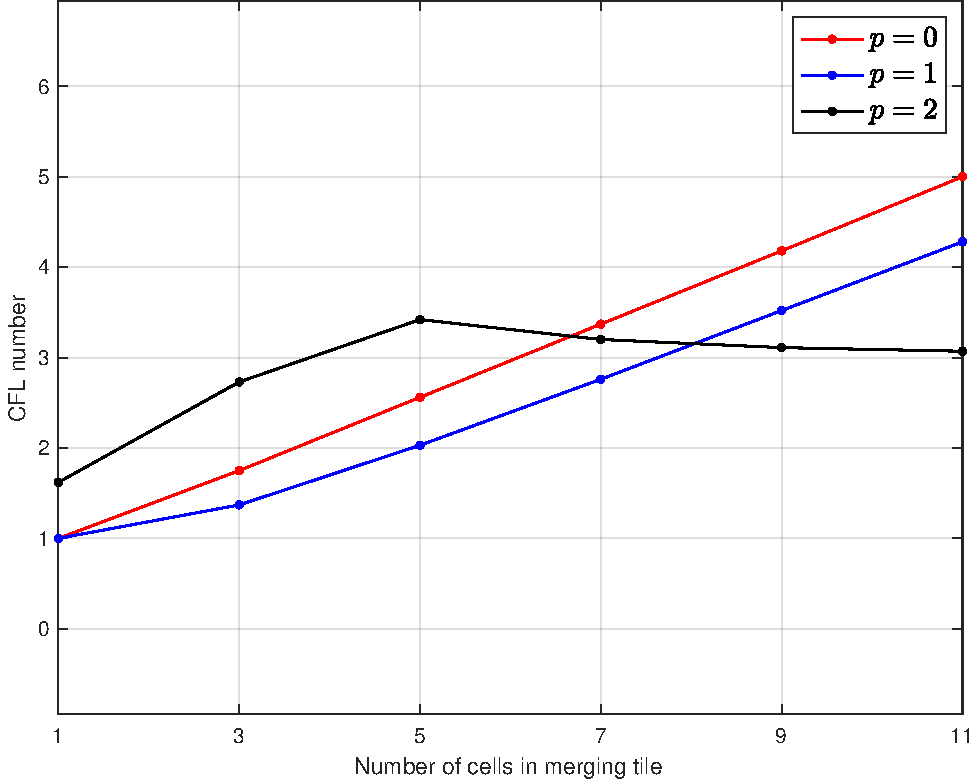
\includegraphics[width=0.45\linewidth]{figs/cflvsj.pdf}} \hfill
\subfloat[CFL versus number of cells in merging tile for various reconstruction stencil widths ($k$).]{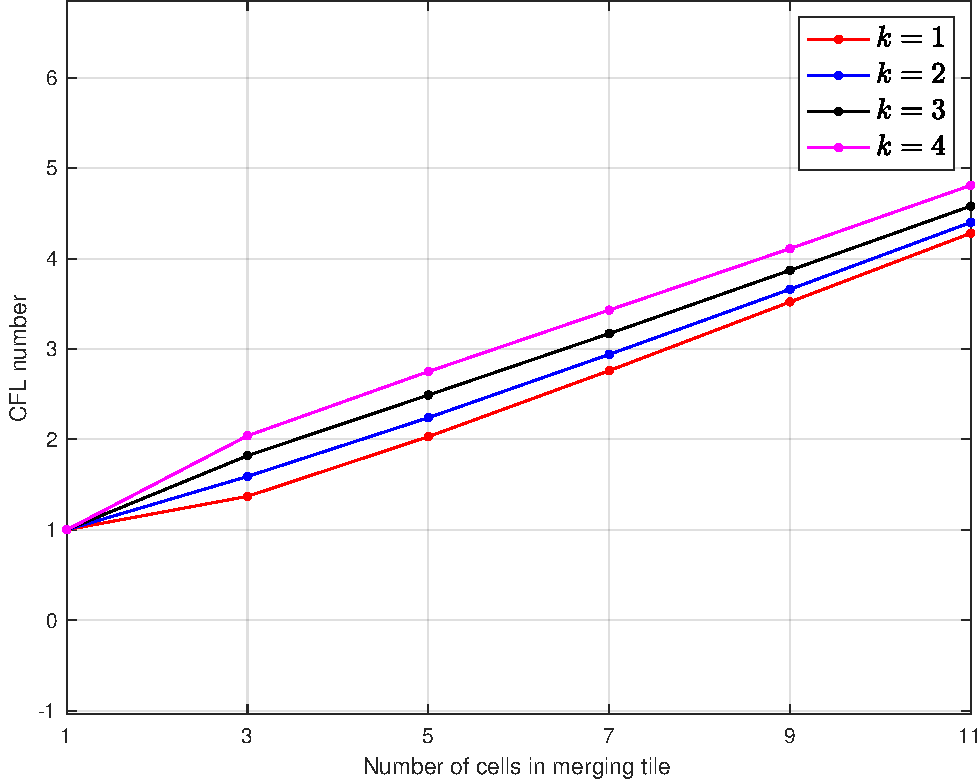
\includegraphics[width=0.45\linewidth]{figs/cflvsk.pdf}}
    \caption{Influence of the merging neighborhood size and the merging tile size on the CFL number.}
    \label{fig:cflvsj}
\end{figure}



% \subsubsection*{Error versus merging neighborhood size}

\subsection{GKS Stability}


\begin{figure}
    \centering
    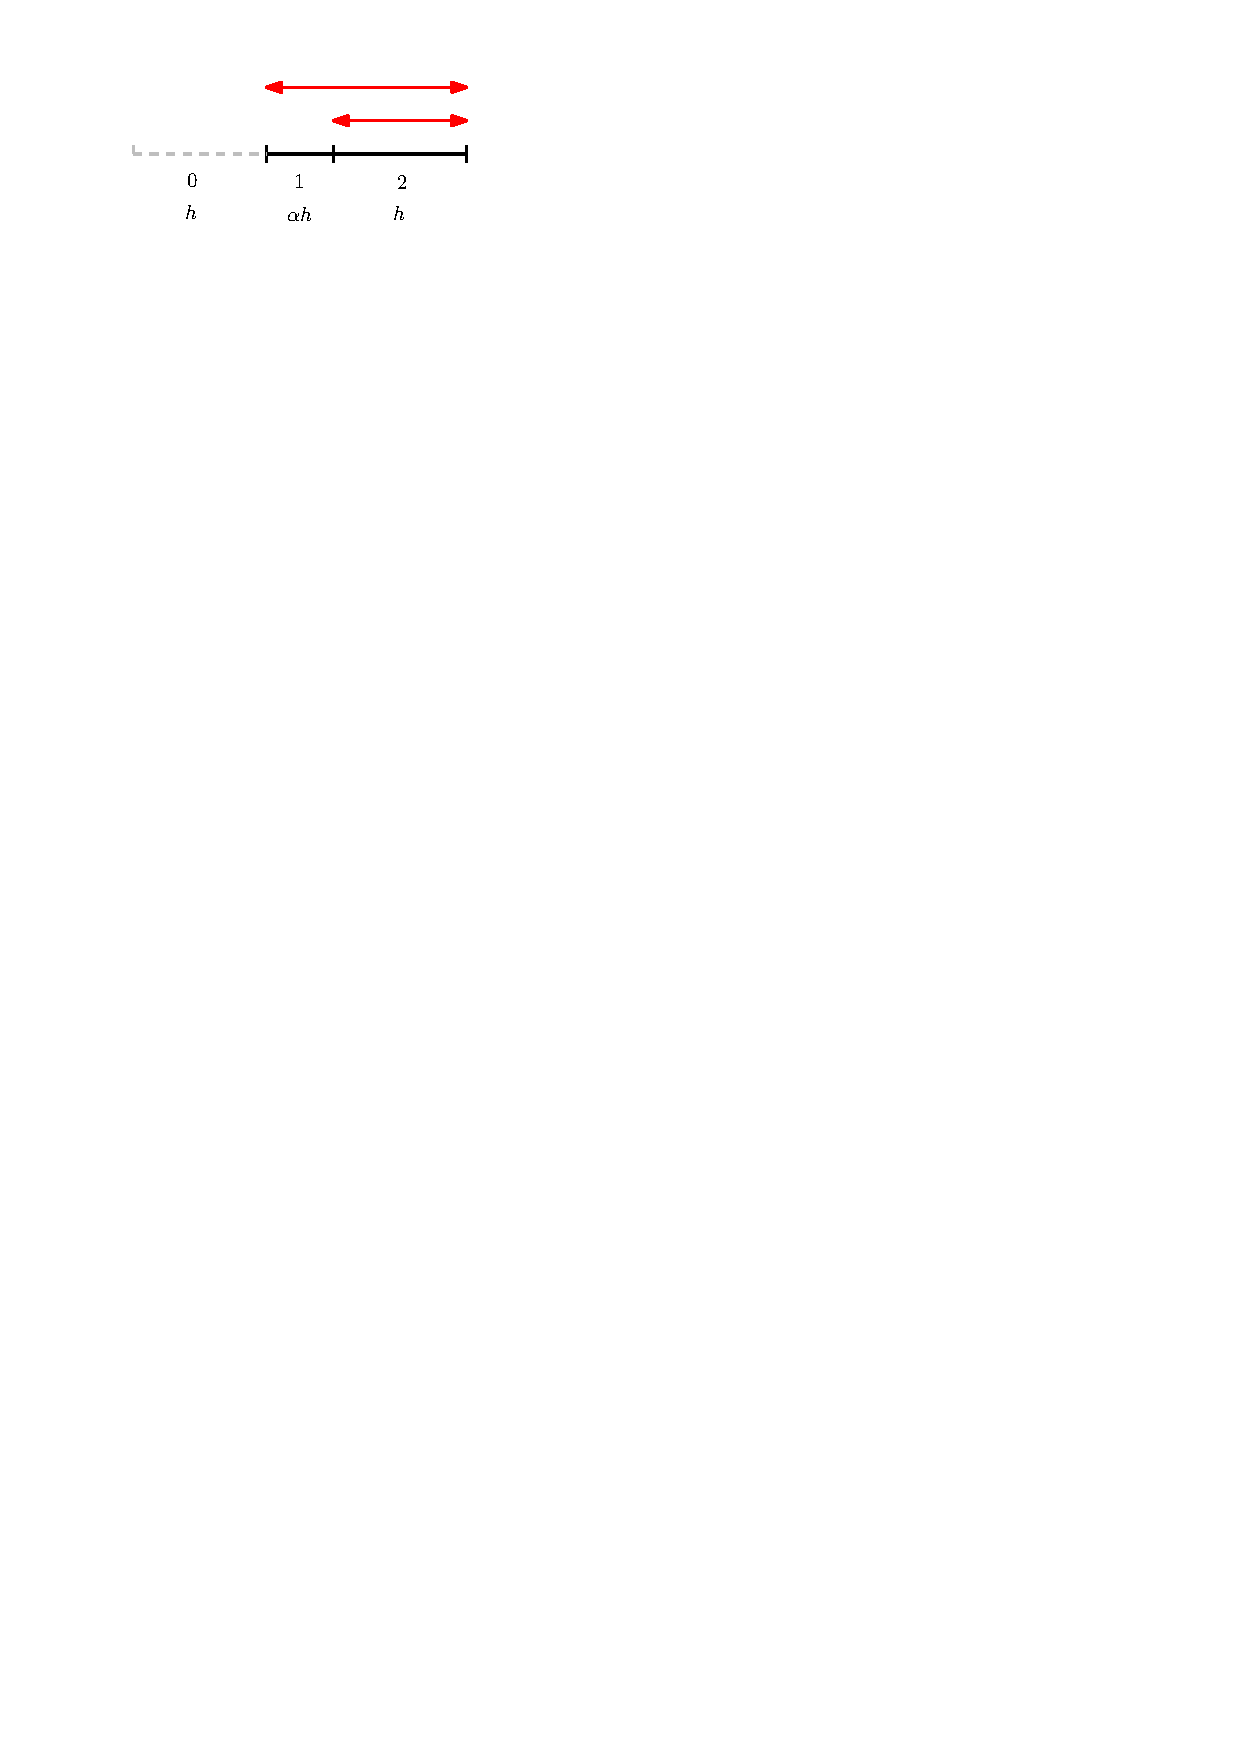
\includegraphics{figs/consistency.pdf}
    \caption{}
    \label{fig:consistency}
\end{figure}


